\documentclass[report]{IEEEtran}

\usepackage{amsmath,graphicx,listings,blindtext,etoolbox}

\makeatletter
\def\do#1{\patchcmd{#1}{\thepage}{\null}{}{\GenericWarning{}{Could not patch \string#1}}}
\docsvlist{\@oddhead,\@evenhead,\ps@headings,\ps@IEEEtitlepagestyle,\ps@IEEEpeerreviewcoverpagestyle}
\makeatother

\newcommand{\inv}[1]{\dfrac{1}{#1}}
\newcommand{\e}[1]{\times 10^{#1}}

\begin{document}
	
	\title{Project 4 - Noise Reduction System}
	\author{Jun D. Ouyang \and \\Guangliang Wu }
	\maketitle
	
	\begin{abstract}
		This project involves the design of a noise reduction system comprised of a pre-emphasis filter and a de-emphasis filter. For this project, we will be designing higher-order active filter circuits using op-amps, and perform a cost analysis of our circuit.
	\end{abstract}
	\section{Objective}
		\subsection{Pre-Emphasis Filter}
			\begin{itemize}
				\item{Design a Pre-emphasis filter which the output at frequencies 100 Hz and 10 kHz must be within $\pm 3$ dB of the input x(t), and the output at frequency range 500 Hz to 2 kHz must be bigger than 20 dB.}
				\item{Design the circuit with entirely with active circuits, but no inductors.}
				\item{Construct the pre-emphasis filter, and then take the gain measurements over the 100 Hz to 10 kHz. }
				\item{Covert the gain to dB, then sketch a plot of gain in dB against frequency on a log scale, then compare the plot with the SPICE results.}
				\item{Analysis the cost of our circuit.}
				\item{Determine the legitamacy of our design.}
			\end{itemize}
		\subsection{De-Emphasis Filter}
			\begin{itemize}
				\item{Design a De-emphasis filter which the output at frequencies 100 Hz and 10 kHz must be within $\pm 3$ dB of the input x(t), and the output at frequency range 500 Hz to 2 kHz must be less than -20 dB.}
				\item{Design the circuit with entirely with active circuits, but no inductors.}
				\item{Construct the de-emphasis filter, and then take the gain measurements over the 100 Hz to 10 kHz. }
				\item{Covert the gain to dB, then sketch a plot of gain in dB against frequency on a log scale, then compare the plot with the SPICE results.}
				\item{Analysis the cost of our circuit.}
				\item{Determine the legitamacy of our design.}
			\end{itemize}
		\subsection{Noise Reduction System}
			\begin{itemize}
				\item{Combine Pre-emphasis and De-emphasis filter together. }
				\item{Construct the combination of Pre-emphasis and De-emphasis we designed, and then take the gain measurements over the 100 Hz to 10 kHz.}
				\item{Cover the gain to dB, then sketch a plot of gain in dB against frequency on a log scale, then compare the plot with the SPICE results.}
				\item{Determine the legitamcy of our final design.}
			\end{itemize}
	
	\section{Specification}
		In designing our circuit we realized two utmost important point in which our circuit has to meet.
		\begin{enumerate}
			\item \label{spec:res:range} We must obtain approximately 0 dB at 100Hz and 10kHz for both the pre-emphasis and the de-emphasis circuit.
			\item \label{spec:res:pg} We must make sure the pre-emphasis filter must be less having at least 20dB more over other values outside the range of 500Hz and 2kHz.
			\item \label{spec:res:output} We must make sure the final cascaded product is within $\pm 3$ dB for our simulation; and due to technical difficulties, $\pm 5$ dB for the experimental output over the range between 100Hz and 10kHz.
		\end{enumerate}
		
		To satisfy \ref{spec:res:range} and \ref{spec:res:pg}, we can use high pass and low pass Butterworth filter circuits by calculating the desired transition slope and scale to the final desired frequencies. Then in the case of the pre-emphasis filter, we can cascade the high pass and low pass circuits together to form a band pass filter with desired gain; and as in the case of the de-emphasis, we will also perform the exact same procedure but instead of cascading, we will be summing the low pass and high pass filters to form a band reject filter with exactly the opposite gain of the pre-emphasis stage.
		
		\subsection{Pre-emphasis Stage}
			In the design of the pre-emphasis stage, we will be cascading a high pass and a low pass filter together and lastly feed through a inverting amplifier to achieve desired gain.
			
			\subsubsection{High Pass Filter}
				To create the abovementioned circuit, we must first calculate the desired slope. We have done so with the following formula directly from the textbook:
				\begin{equation}
					\label{spec:hp:eq:n}
						n=\dfrac{
							\log{\left(
								\dfrac{
									\sqrt{10^{-0.1A_s}-1}
								}{
									\sqrt{10^{-0.1A_p}-1}
								}
							\right)}}{
							\log{
								(\omega_p / \omega_s)
							}
						}
				\end{equation}
				
				Because we want at 100 Hz about 0 dB and at 500 Hz about 20 dB, we can set the cutoff frequency of the high pass filter to be at 500 Hz, where $A_s = -23$ dB, $A_p = -3$ dB, $\omega_s=100$ Hz, and $\omega_p=500$ Hz. We can then scale the amplitude by 23 dB (approximately $10^{23/20} = 14.1 $ dB to achieve our specification. Using such values and via \eqref{spec:hp:eq:n}, we obtain the following,
				\begin{align*}
					n&=\dfrac{
						\log{\left(
							\dfrac{
								\sqrt{10^{-0.1\times (-23)}-1}
							}{
								\sqrt{10^{-0.1\times (-3)}-1}
							}
						\right)}}{
						\log{
							(500 / 100)
						}
					} \\
					&\approx 1.64
				\end{align*}
				Because we can only have integer value of $n$, we must either ceil or floor the calculated value. Since the value is closer to 2 dB, and since the BW filter guaranteed to pass through 500 Hz at -3 dB after frequency scaling, we chose to ceil the calculated $n$ in the hopes to preserve the $\pm 3$ dB boundary of the original input signal at 100 Hz. Therefore, we obtain after ceiling,
				\begin{equation}
					\label{spec:hp:n}
					n=2
				\end{equation}
				
				Now we can build the high pass stage with the $n=2$ (second order) Butterworth high pass filter. The second order BW high pass filter has the s-domain equation:
				\begin{equation}
					\label{spec:bw:hp:n2}
					H(s)=\dfrac{s^2}{s^2+\dfrac{2}{R_2~C}~s+\inv{R_1~R_2~C^2}}
				\end{equation}
				The circuit for the second order BW HP filter is as follows:
				\begin{figure}[h!]
					\begin{center}
						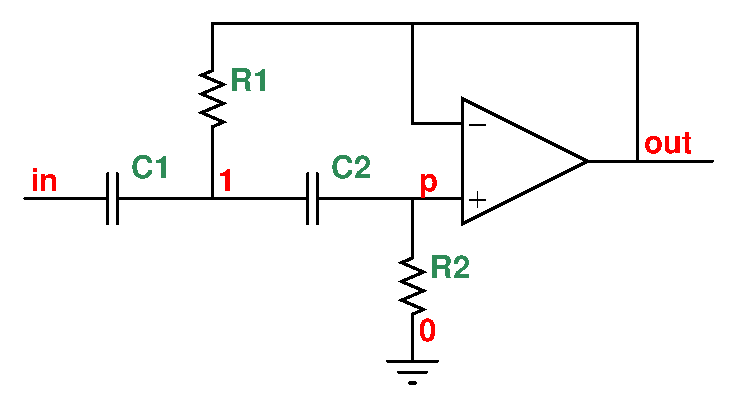
\includegraphics[width=250px]{hp.eps}
					\end{center}
				\end{figure}
				
				Note, in this case, $C_1=C_2=C$, and this circuit has cutoff frequency at $\omega_c = \inv{R^2~C_1~C_2} = 500 Hz \times 2~\pi = 1000~\pi rad/s$. But as off now, its unscaled version has only $\omega_c = 1 rad/s$ as R's and C's are in values of prototype circuit of 1 $\Omega$ and 1 $F$ respectively.
				
			\subsubsection{Low Pass Filter}
				For the low pass stage of the pre-emphasis filter, we may apply the same concept to the high pass filter to find the suitable BW order for the slope between $\omega_p=2$~kHz, $\omega_s=10$~kHz, $A_p=-3$~dB, and $A_s=-23$~dB. We apply the low-pass BW order formula below, 
				\begin{equation}
					\label{spec:lp:eq:n}
						n=\dfrac{
							\log{\left(
								\dfrac{
									\sqrt{10^{-0.1A_s}-1}
								}{
									\sqrt{10^{-0.1A_p}-1}
								}
							\right)}}{
							\log{
								(\omega_s / \omega_p)
							}
						}
				\end{equation}
				Obtaining,
				\begin{align*}
					n&=\dfrac{
						\log{\left(
							\dfrac{
								\sqrt{10^{-0.1\times (-23)}-1}
							}{
								\sqrt{10^{-0.1\times (-3)}-1}
							}
						\right)}}{
						\log{
							(10000 / 2000)
						}
					} \\
					&\approx 1.64
				\end{align*}
				Therefore, we will also choose second order BW filter as we did with the high pass stage. The second order low-pass BW filter has the following s-domain frequency response:
				\begin{equation}
					\label{spec:bw:lp:n2}
					H(s)=\dfrac{1/(R^2~C_1~C_2)}{s^2+\dfrac{2}{R~C_1}~s+\inv{R^2~C_1~C_2}}
				\end{equation}
				The circuit for the second order BW LP filter is as follows:
				\begin{figure}[h!]
					\begin{center}
						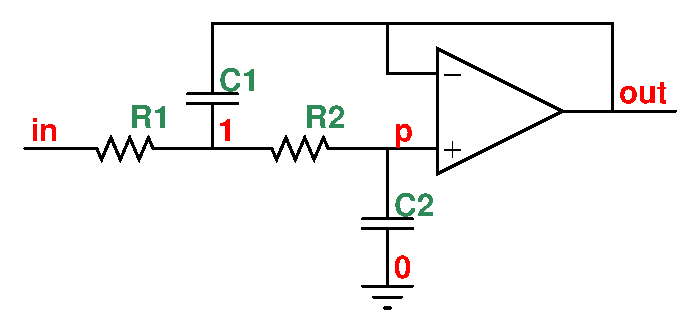
\includegraphics[width=250px]{lp.eps}
					\end{center}
				\end{figure}
				
				With $\omega_c = \tfrac{1}{R^2~C_1~C_2}$.
			\subsubsection{Gain stage}
				The pre-emphasis must employs a gaining stage to have its values above 0 dB. Using an inverting op-amp configuration in such case proves to be most direct approach. It has simple transfer function of $H(j\omega) = -\tfrac{R_f}{R_i}$. Its schematics is shown below:
				\begin{figure}[h!]
					\begin{center}
						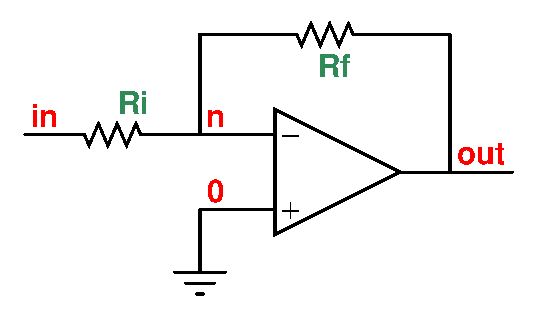
\includegraphics[width=200px]{gain.eps}
					\end{center}
				\end{figure}
			
			By cascading the high pass stage, low pass stage and the gain stage in series, will therefore satisfy our specification. Its final product is not shown here as it is easy to imagine. But, as usual, its transfer function, on the other hand, can be calculated by multiplying abovementioned filters' frequency responses. The final transfer function for the pre-emphasis filter is therefore:
			
			\begin{align}
				H(s) = & H_{hp}(s)~\times~H_{lp}(s)~\times~H_{gain}(s) \\
				= & \dfrac{s^2}{s^2+\dfrac{2}{R_2~C}~s+\inv{R_1~R_2~C^2}} \\ & \times \dfrac{1/(R^2~C_1~C_2)}{s^2+\dfrac{2}{R~C_1}~s+\inv{R^2~C_1~C_2}} \times \dfrac{R_f}{R_i}
			\end{align}
			
			As usual, the center frequency of any bandpass filter is,
			\begin{equation}
				\omega_o = \sqrt{\omega_{c_{hp}} \omega_{c_{lp}}} = \sqrt{\inv{R_1~R_2~C^2} \times \inv{R^2~C_1~C_2}}
			\end{equation}
			
			To view the full connection of the pre-emphasis filters, see appendix A.
		
		\subsection{De-emphasis Stage}
			The design of the de-emphasis stage is quite tricky because we cannot simply just rely on the 100Hz and 500Hz or the 2kHz and 10kHz pair, because if we employed frequency scaling to such places, the slope of the frequency response of the pre-emphasis does not match with that of the de-emphasis. Therefore, we must scale the de-emphasis stage quite differently. But, however, we note that however we might change the cutoff frequency by scaling, the general slope however, does not need to be or mustn't be altered to cancel out the slope of the pre-emphasis filter; and it is precisely this, we can apply the same filter components in the pre-emphasis stage. But this time, instead of building a band-pass filter, we must build a band-reject filter because we need to undoes the amplification created by the pre-emphasis filter. Therefore, when we combine the two low pass and high pass filters, we do not cascade them in series but in parallel and have their corresponding output signals summed up to create a band pass filter. In case of exceptions, we can also throw in another inverting op-amp to adjust to the adequate  signal level. Therefore, the de-emphasis requires four building blocks: a BW LP filter, a BW HP filter, a summing amplifier, and possibly an inverting op-amp.
			
			\subsubsection{Low-pass Stage}
				This stage, as its name indicates, undergoes a low-pass filter. It has exactly the same identical structure of the \eqref{spec:bw:lp:n2} and therefore we will omit its discussion here. The only difference will be its scaling, which will be discussed at length in the simulation section because the calculations done by idealization of the circuit elements is prone to have errors. This low pass stage will actually have $K_f$ scaling the prototype cutoff frequency to around 100Hz.
				
			\subsubsection{High-pass Stage}
				The high pass stage equivalent to the pre-emphasis high pass filter with equation \eqref{spec:bw:hp:n2}, except having its frequency scaled to having $\pm 3$dB at around 10kHz.
			
			\subsubsection{Sum Stage}
				The summing op-amp is simply the standard unity gain summing op-amp configuration with $H(s)=1$. Its setup is shown below:
				\begin{figure}[h!]
					\begin{center}
						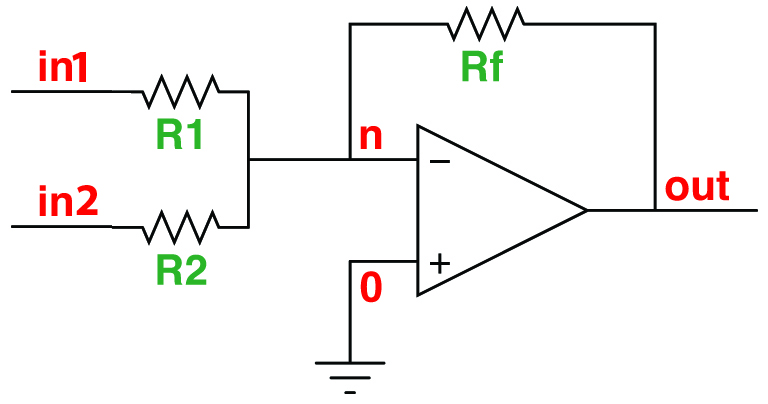
\includegraphics[width=200px]{sum.jpg}
					\end{center}
				\end{figure}
				
			Where $R_1 = R_2 = Rf$ since it is unity gain.
			
			\subsection{Gain stage}
				We cannot expect any kind of possible disturbance caused by the non-ideality of the op-amp model during simulation and/or experiment. We must therefore allow an extra inverting amplifier in our arsenal to adjust the amplitude of the resulting wave as needed. The inverting op-amp is exactly the same as the one from the pre-emphasis stage. We therefore will not discuss of it.
				
			We can now combine all these elements together into the de-emphasis configuration. It ultimately ends up as the following circuit diagram:
			
			Its transfer function is:
			\begin{align}
				H(s) = & H_{hp}(s)~\times~H_{lp}(s)~\times~H_{gain}(s) \\
				= & \Bigg( \dfrac{s^2}{s^2+\dfrac{2}{R_2~C}~s+\inv{R_1~R_2~C^2}} \\ & + \dfrac{1/(R^2~C_1~C_2)}{s^2+\dfrac{2}{R~C_1}~s+\inv{R^2~C_1~C_2}} \Bigg) \times \dfrac{R_f}{R_i}
			\end{align}
			
			As usual, the center frequency of any bandreject filter is the same as that of the bandpass filter,
			\begin{equation}
				\omega_o = \sqrt{\omega_{c_{hp}} \omega_{c_{lp}}} = \sqrt{\inv{R_1~R_2~C^2} \times \inv{R^2~C_1~C_2}}
			\end{equation}
			
			The only difference between the bandpass of the pre-emphasis stage and the bandreject of the de-emphasis stage is their frequency scaling value and the way components of LP and HP filters connecting together as shown by the above equations. To view the full connection of the de-emphasis filters, see appendix B.
		
	\section{Simulation}
		In simulating this nrs circuit, we broke down the entire spice code bit by bit and encompassed automatic expression evaluation to facilitate us from the burden of scaling capacitors or resistors values. Therefore, instead of focusing on how we scale here, we would be able to focus on how we could achieve our specification.
		
		\subsection{The Ingredients}
		Before we begin explaining our code listings, we will inform this report's reader that our project's source code is available online at GitHub in this following address:
		\begin{center}
			http://www.github.com/jouyang3/nrs
		\end{center}
		
		Now onto the simulation subject. Because the reusability of the second order low pass and high pass sub-circuit, we were able to parametrize both low pass and high pass sub-circuit to avoid code duplication. The resulting code listing for the low-pass filter is hence as follows in the file lp.cir:
		\begin{center}
		\begin{lstlisting}[caption=2nd order BW LP netlist.][h!]
.SUBCKT lp in out kf=1 r=1
.PARAM km=r
R1	in	1	R=r
R2	1	p	R=r
C1	1	out	C='1.414/km/kf'
C2	p	0	C='0.707/km/kf'
X1	p	out	out	popamp
.ENDS lp
		\end{lstlisting}
		\end{center}
		Here, we enabled the low pass filter accept scaling argument thus we were able to alter the frequency scaling as needed both by the pre-emphasis and the de-emphasis stage. The expression of $C_1$ and $C_2$ enabled automatic scaling when the scaling factor $K_f$ sets in (by default, there's no scaling, hence $K_f=1$. The circuit with nodes labeled for this LP netlist is reprinted here at the reader's convenience.
		\begin{center}
			\begin{figure}[h!]
					\label{lp.cir}
					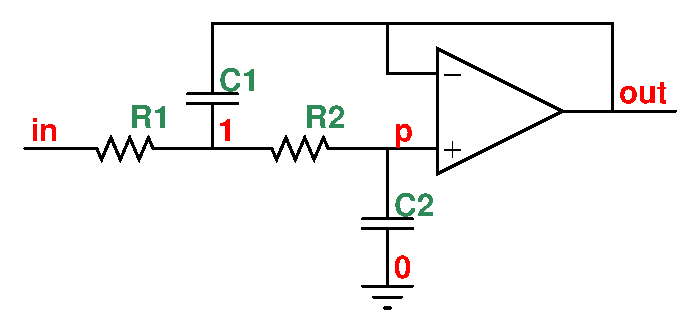
\includegraphics[width=250px]{lp.eps}
					\caption{Second order BW LP Circuit.}
			\end{figure}
		\end{center}
		We applied the same treatment to the high pass netlist. Here's its netlist:
		\begin{center}
		\begin{lstlisting}[caption=2nd order BW HP netlist.][h!]
.SUBCKT hp in out kf=1 c=1
.PARAM km='1/kf/c'
C1	in	1	C=c
R1	1	out	R='km*0.707'
C2	1	p	C=c
R2	p	0	R='km*1.414'
X1	p	out	out	popamp
.ENDS hp
		\end{lstlisting}
		\end{center}
		And again, reprinting the circuit here to cross-reference by the reader:
		\begin{center}
			\begin{figure}[h!]
					\label{hp.cir}
					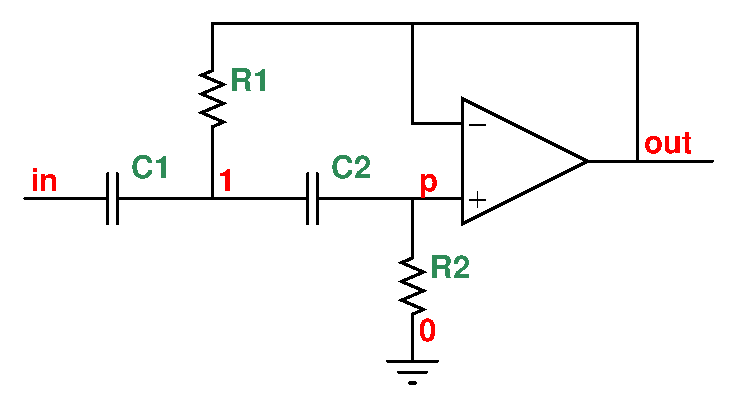
\includegraphics[width=250px]{hp.eps}
					\caption{Second order BW HP Circuit.}
			\end{figure}
		\end{center}
		Notice that, instead of scaling the capacitor, per the textbook, we needed to scale the value of the resistors, and that is what we've done.
		
		And we did exactly the same just with the inverting op-amp so that it accepts a scaling coefficient:
		\begin{center}
		\begin{lstlisting}[caption=Inverting Op-Amp netlist.][h!]
.SUBCKT	gain in out a=1
* K=27.67dB
Rf	n	out	R=(a*1k)
Ri	in	n	1k
X1	0	n	out	popamp
.ENDS gain
		\end{lstlisting}
		\end{center}
		and its circuit diagram:
		\begin{figure}[h!]
			\label{gain.cir}
			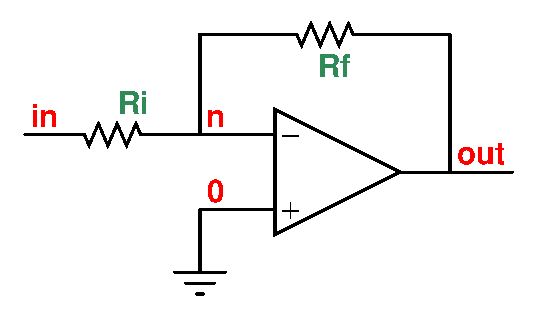
\includegraphics[width=250px]{gain.eps}
			\caption{Inverting Op-amp Circuit.}
		\end{figure}
		
		Notice the reference of a popamp sub-circuit, it is actually a fun way to say "Pseudo-opamp", its netlist came directly from Project 3 and we will also include it below:
		\begin{center}
		\begin{lstlisting}[caption=RC Pseudo-op-amp netlist.][h!]
.SUBCKT popamp 	4 	n 	2
Ri	4	n	2MEG
Ei	1	0	4	n	1
R	1	3	1
C	3	0	0.03183
Eo	6	0	3	0	200K
Ro	6	2	75
.ENDS popamp
		\end{lstlisting}
		\end{center}
		Note that this op-amp accepts three nodes, the first being the non-inverting input, the second the inverting and the last to be the output node. We will not show the pseudo op-amp circuitry in here because it diverts from our purpose of investigating noise reduction system.
		
		The last part of the puzzle is the summing amplifier applied by the band-reject filter of the de-emphasis filter. Here's its netlist:
		\begin{center}
		\begin{lstlisting}[caption=Summing Op-Amp netlist.][h!]
.SUBCKT sum in1 in2 out
R1	in1	n	10k
R2	in2	n	10k
Rf	n	out	10k
X1	0	n	out	popamp
.ENDS sum 
		\end{lstlisting}
		\end{center}
		and its circuit diagram:
		\begin{figure}[h!]
			\label{sum.cir}
			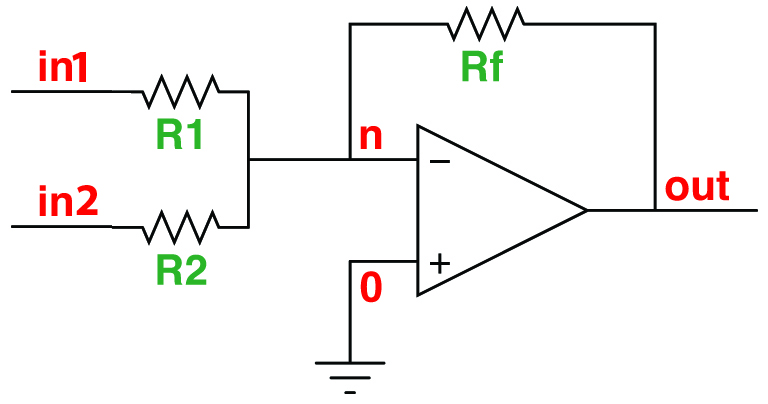
\includegraphics[width=250px]{sum.jpg}
			\caption{Summing Op-amp Circuit.}
		\end{figure}

	\subsection{Pre-emphasis}
		Now we are ready to build our pre-emphasis netlist:
		\begin{center}
		\begin{lstlisting}[caption=Pre-emphasis netlist.][h!]
.SUBCKT preemp in out
.PARAM khf='2*530*Pi'
.PARAM klf='w0^2/khf'
Xhp	in	1 hp kf=khf	c=2n
Xlp	1	2 lp kf=klf 	r=120k
Xg	2	out gain a='10^(29/20)'
.ENDS preemp
		\end{lstlisting}
		\end{center}
		its diagram is:
		\begin{figure}[h!]
			\label{preemp.cir}
			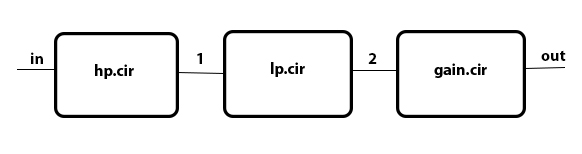
\includegraphics[width=250px]{preemp-sim.jpg}
			\caption{Pre-emphasis Op-amp Circuit.}
		\end{figure}
		Notice how simple this is. We simply called the high pass and low pass filters and scale it to what we want. In here, after numerous attempts to meet specification, we finally settled on scaling the frequency above 500Hz to 530Hz! This is the only way that it met our spec. One may see the entirety of the pre-emphasis filter in appendix A.
		\linebreak
		\linebreak
		If driven by the test current defined TestPreemp.cir a waveform appears:
		\begin{figure}[h!]
			\label{preemp-plot.cir}
			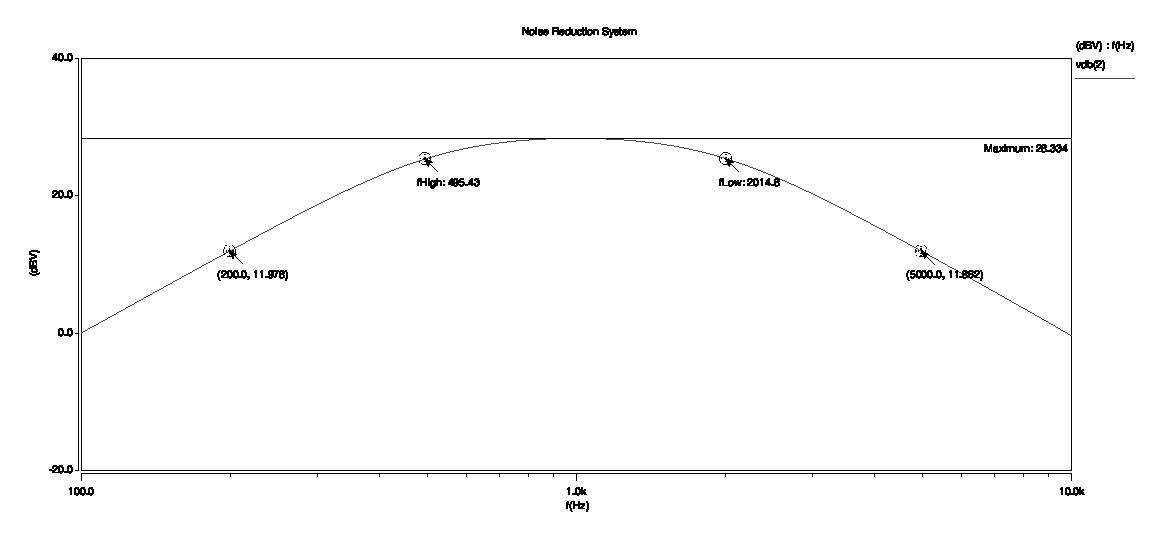
\includegraphics[width=250px]{preemp_plot.eps}
			\caption{Pre-emphasis Op-amp Circuit.}
		\end{figure}
		
		To see the actual data points on the plot, see Appendix C for a larger, and comprehensive view.
	\subsection{De-emphasis}
		Then, we turn our attention to the de-emphasis netlist:
		\begin{center}
		\begin{lstlisting}[caption=De-emphasis netlist.][h!]
.SUBCKT deemp in out
.PARAM klf='2*97*Pi'
.PARAM khf='w0^2/klf'
Xlp	in	1	lp	kf=klf	r=120k
Xhp	in	2	hp	kf=khf	c=2n
Xsum	1	2	3	sum
Xg	3	out	gain	a='10^(3.5/20)'
.ENDS deemp
		\end{lstlisting}
		\end{center}
		If driven by the test current defined TestDeemp.cir a waveform appears:
		\begin{figure}[h!]
			\label{deemp.cir}
			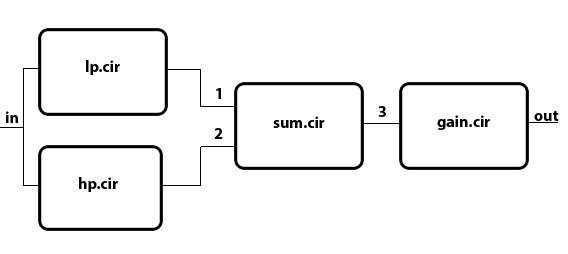
\includegraphics[width=250px]{deemp-sim.jpg}
			\caption{De-emphasis Op-amp Circuit.}
		\end{figure}
		
		We will also present you with a glimpse of its general waveform (again turn to Appendix C for help if you wish to know more.
		\begin{figure}[h!]
			\label{deepm-plot.cir}
			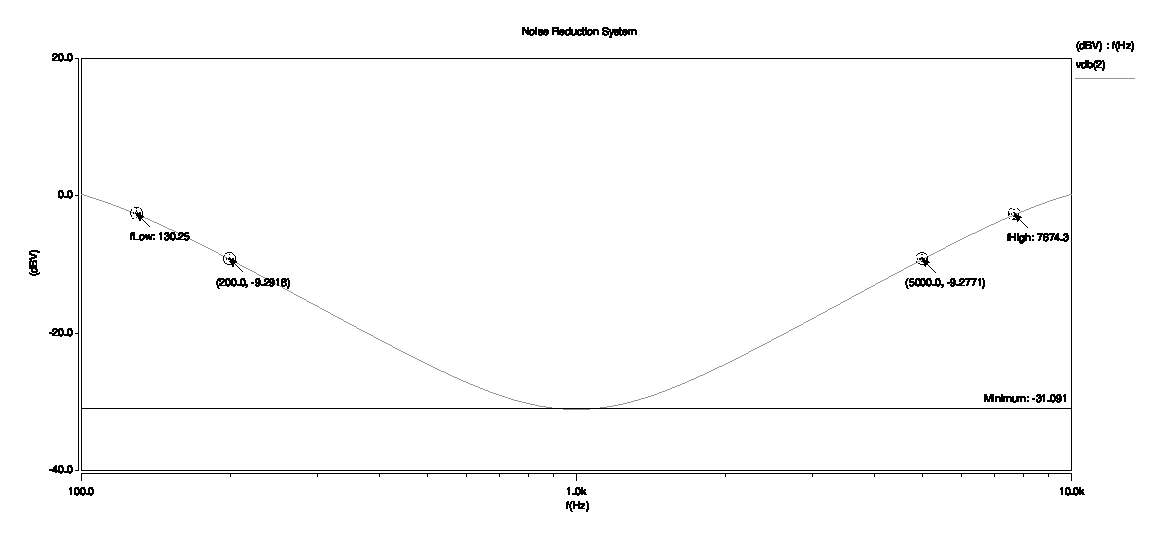
\includegraphics[width=250px]{deemp_plot.eps}
			\caption{Pre-emphasis Op-amp Circuit.}
		\end{figure}
		
	Now we can finally see the result of the NRS system! And we are going to do it by cascading the two emphasis filters and run AC analysis of the entire circuit!
	
	We begin by cascading the output of the pre-emphasis circuit to the input of the de-emphasis circuit. Here's the diagram when we made such connections:
	\begin{figure}[h!]
		\label{nrs.cir}
		\begin{center}
			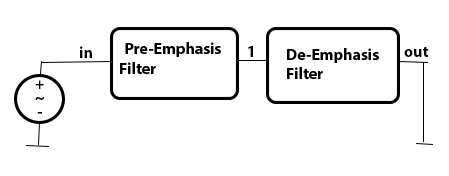
\includegraphics[width=250px]{nrs.jpg}
		\end{center}
	\end{figure}
	\newpage
	This is the netlist that we used to connect the two filters and at the same time tested the entire system:
	\begin{center}
		\begin{lstlisting}[caption=NRS netlist.][h!]
Noise Reduction System - Main
.INCLUDE constants.cir
.INCLUDE popamp.cir
.INCLUDE hp.cir
.INCLUDE lp.cir
.INCLUDE gain.cir
.INCLUDE sum.cir
.INCLUDE preemp.cir
.INCLUDE deemp.cir
Vin	0	1	AC	1
Xpe	1	2	preemp
Xde	2	3	deemp
.AC DEC 40 100 10k
.PRINT VDB(3)
.OPTION list
.OPTION post
.END
		\end{lstlisting}
		\end{center}
		
	Notice in this circuit, we are including all of the sub-circuit files that has mutual library dependency for each to function. We have named each file according to their sub-circuit names like the case of writing code in Java. The file constant holds nothing more but these following two constants that is quite crucial to the success of the team. They are:
		\begin{center}
		\begin{lstlisting}[caption=System constants][h!]
.PARAM Pi=3.1415926535897932384626433832\\
795028841971693993751058
.PARAM w0='2000*Pi'
		\end{lstlisting}
		\end{center}
	We have set the value of $\pi$ and the center frequency at $2000\pi$ or 1000Hz.
	Here's the result of the final wave after passing through our N.R.S.:
	\newpage
	\begin{figure}[h!]
		\begin{center}
			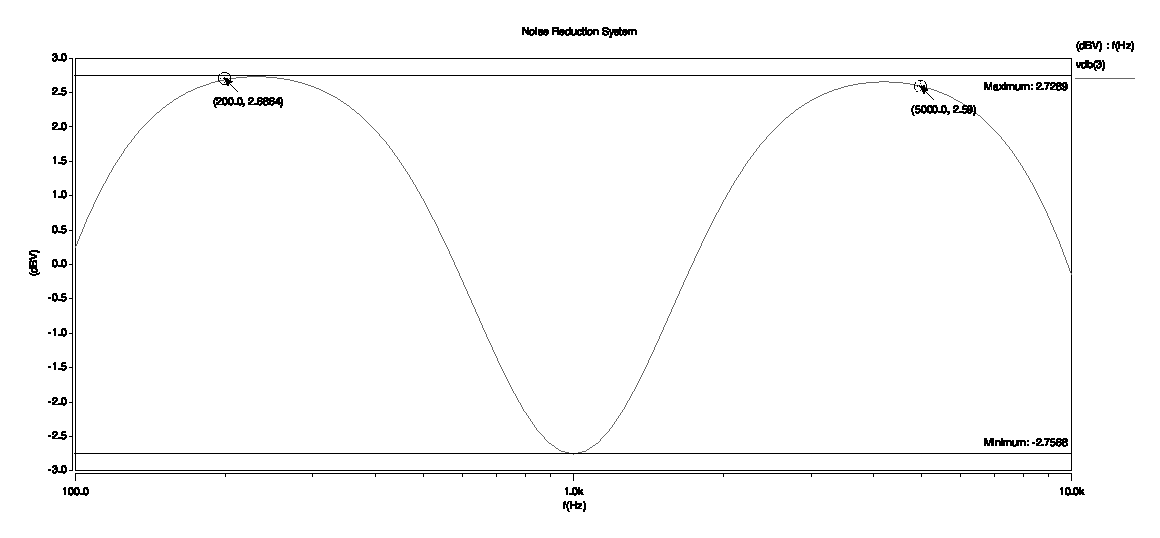
\includegraphics[width=250px]{nrs_plot.eps}
		\end{center}
	\end{figure}
	
	Again, see Appendix C for full treatment of data-craving.
		
		\newpage
		\onecolumn
		\section*{Appendix A: Pre-Emphasis Circuit}
		\it{Warning: nodes with the same name each has different scope. The repetition of the same name does not mean short. Circuit is made to accomodate each subcircuit that comprised the system.}
			\begin{figure}[h!]
				\begin{center}
					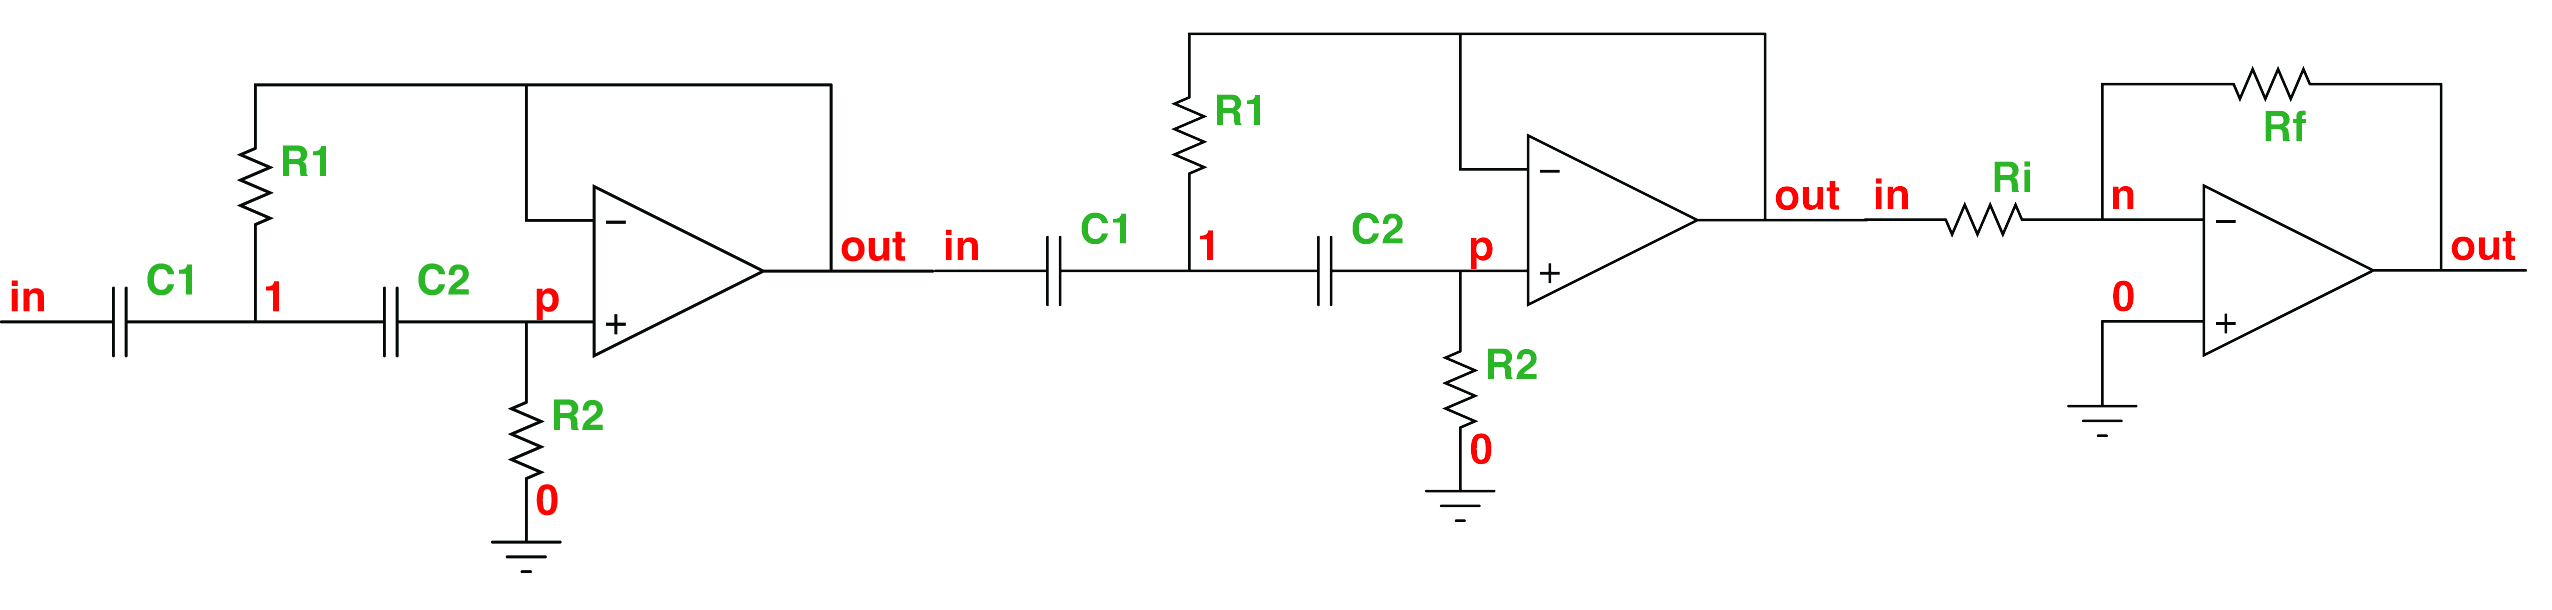
\includegraphics[width=\textwidth]{preemp.jpg} 
				\end{center}
			\end{figure}
		\section*{Appendix B: De-Emphasis Circuit}
		\it{Warning: nodes with the same name each has different scope. The repetition of the same name does not mean short. Circuit is made to accomodate each subcircuit that comprised the system.}
			\begin{figure}[h!]
				\begin{center}
					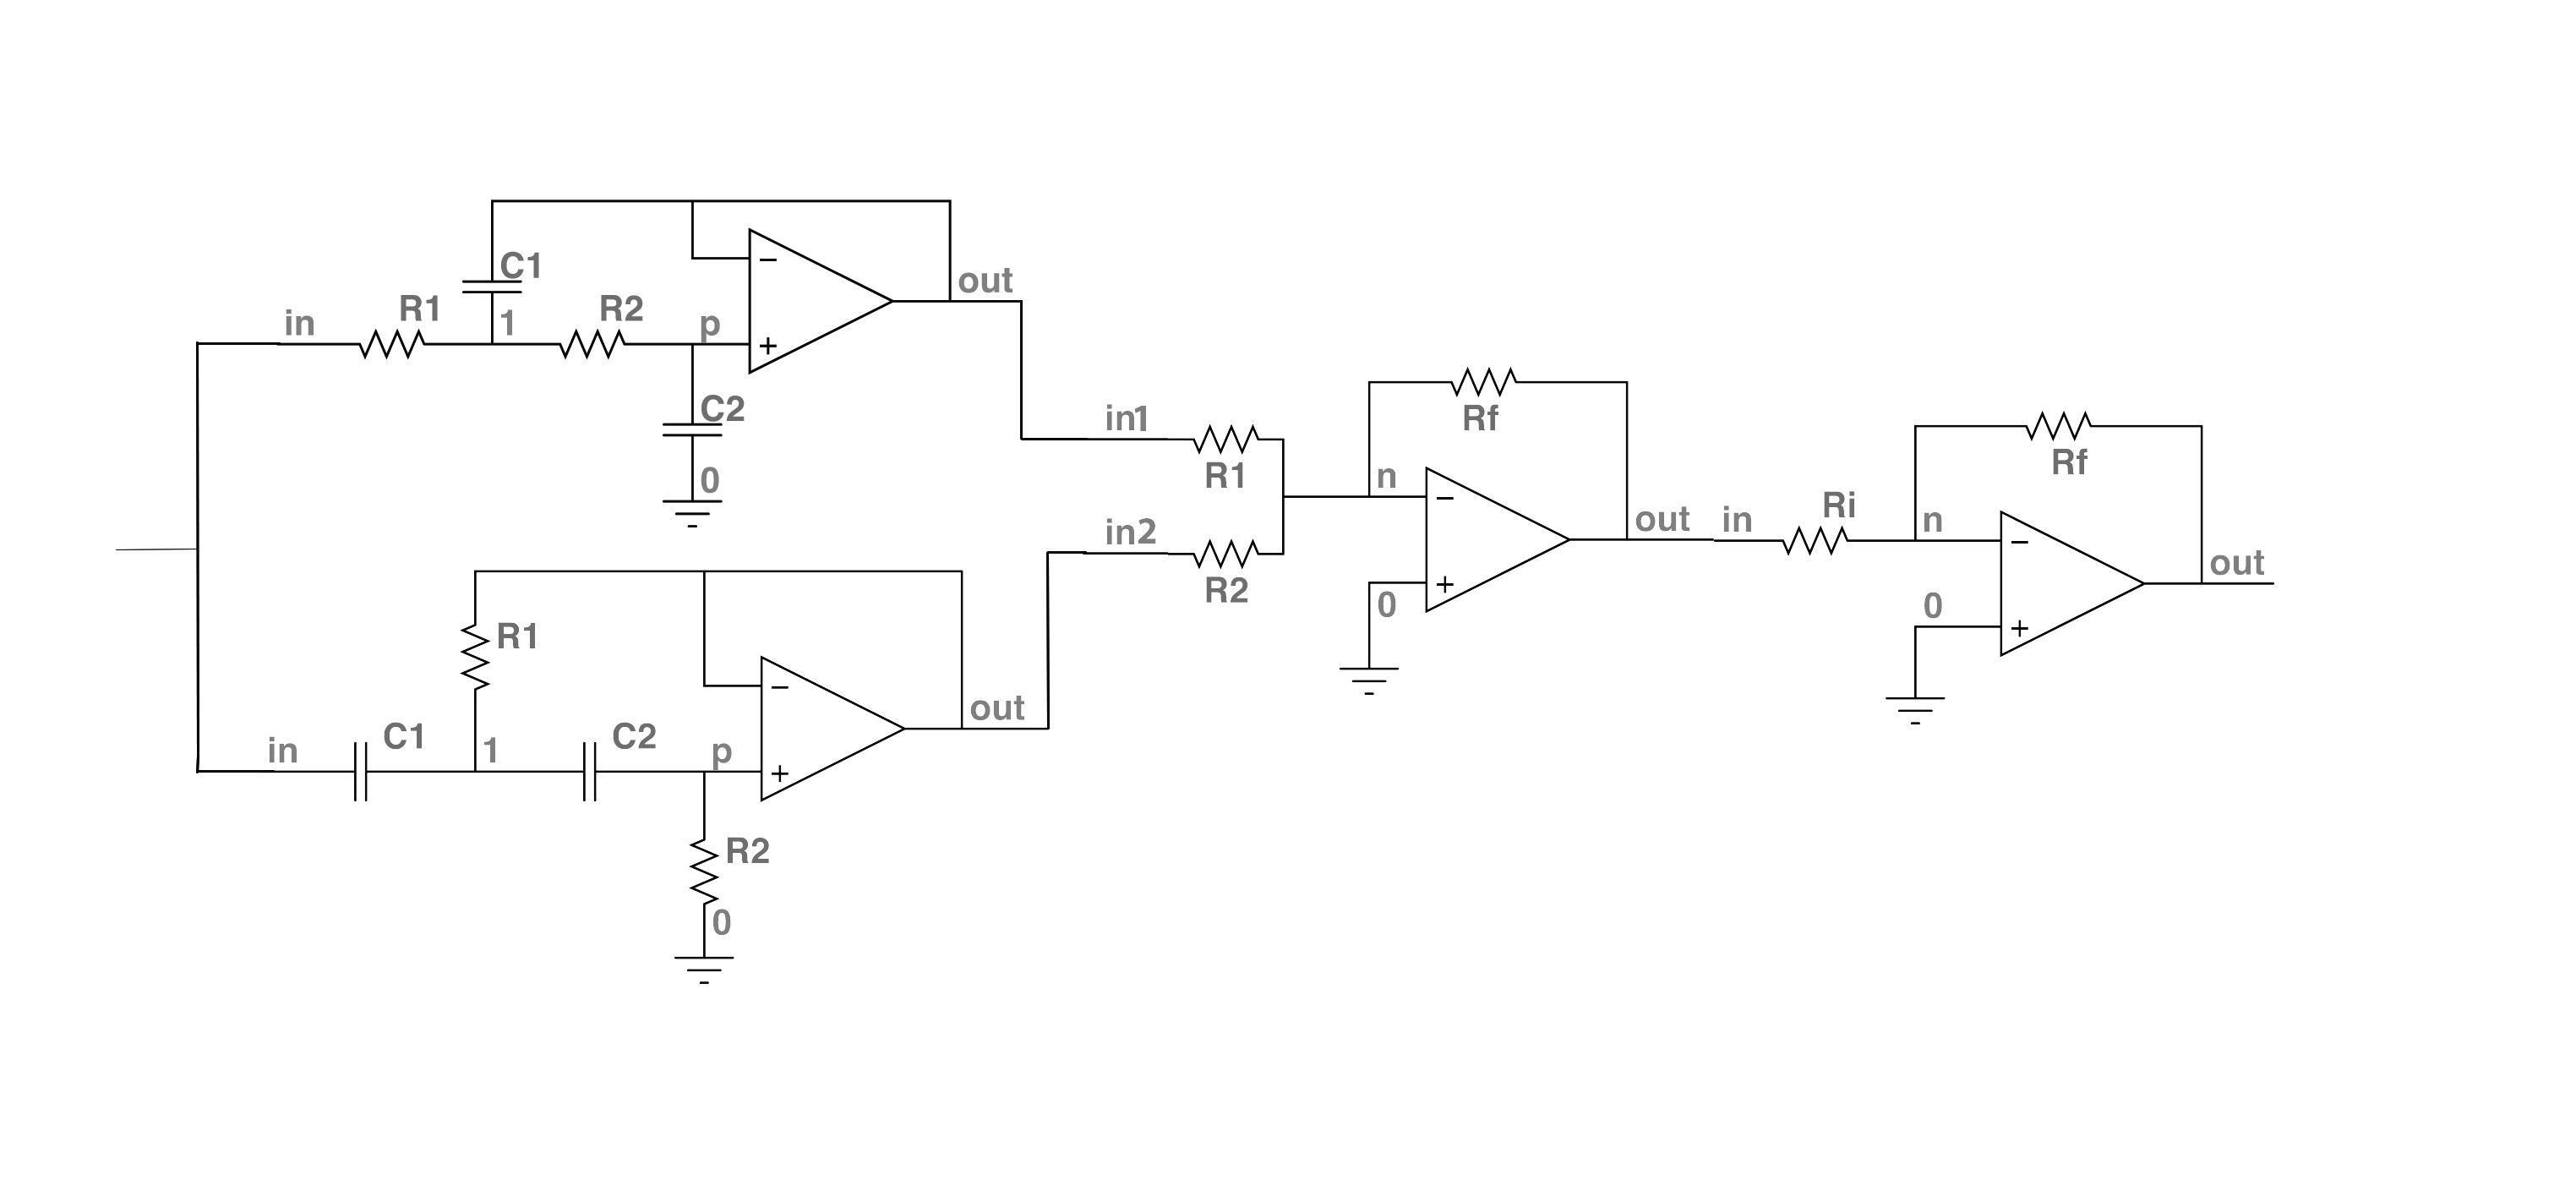
\includegraphics[width=\textwidth]{deemp.jpg}
				\end{center}
			\end{figure}
		\newpage
		\section*{Appendix C: Enlarged Labeled Plots}
			\begin{figure}[h!]
				\begin{center}
					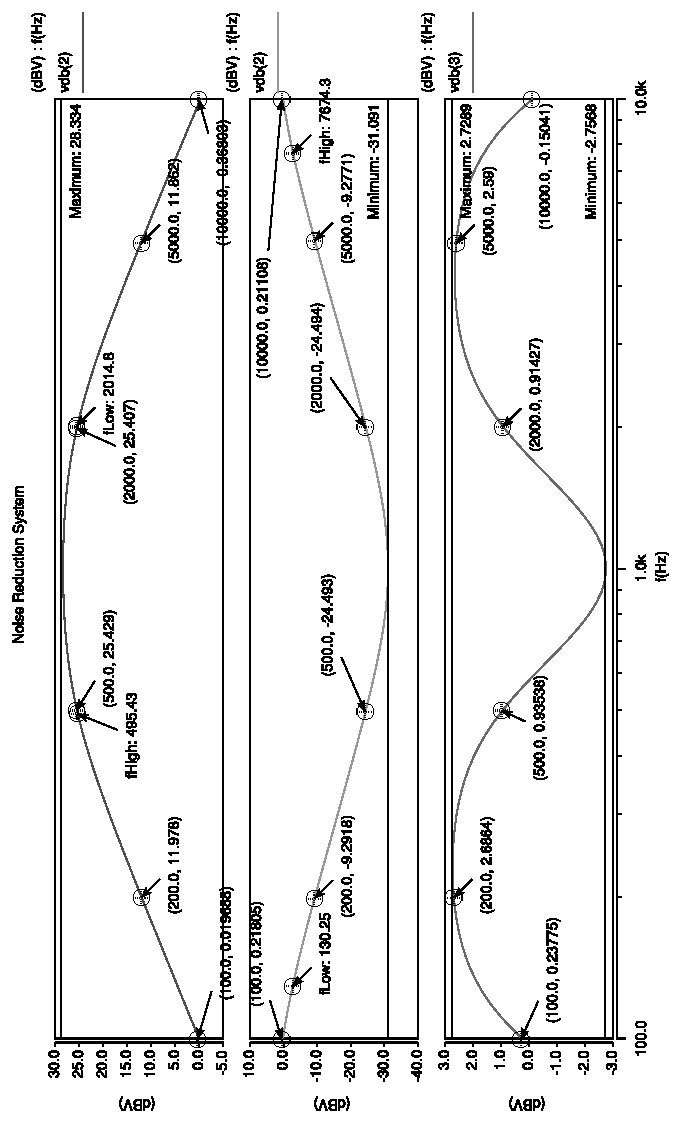
\includegraphics[width=\textwidth,height=650px]{nrs_whole}
				\end{center}
			\end{figure}

\end{document}